\documentclass[pdftex]{beamer}
\usetheme{metropolis}


\usepackage[english]{babel}
\usepackage[latin1]{inputenc}
\usepackage{times}
\usepackage[T1]{fontenc}
\usepackage{fancyvrb}
\usepackage{listings}
\begin{document}
\lstset{language=C, escapeinside={(*@}{@*)}, numbers=left,
  basicstyle=\tiny, showspaces=false, showtabs=false, showstringspaces=false}

\title{A Look Inside FreeBSD with DTrace}
\subtitle{Processes}
\author[shortname]{George V. Neville-Neil \and Robert N. M. Watson}

\begin{frame}
  \titlepage
\end{frame}

\begin{frame}
  \frametitle{The Process Model}
  \begin{itemize}
  \item The most basic container
  \item All of a program's resources
  \item The entity that is scheduled and executed
  \end{itemize}
\end{frame}

\begin{frame}[fragile]
  \frametitle{The UNIX process life cycle}

  \begin{columns}[T]
    \column{0.5\textwidth}
      \vspace{0.5cm}
      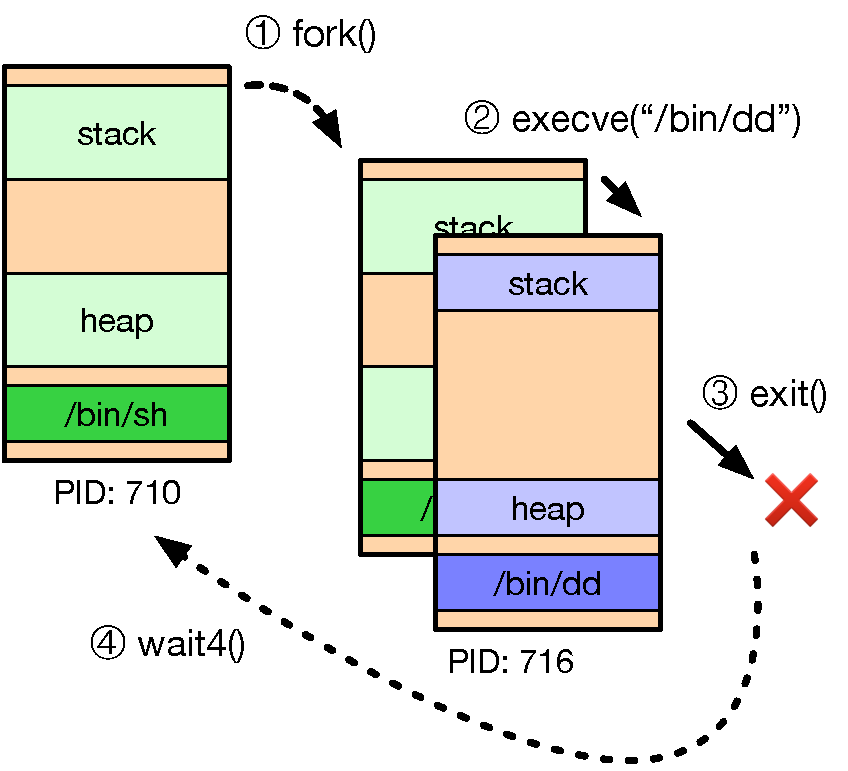
\includegraphics[width=\textwidth]{../figures/process-life-cycle.pdf}

    \column{0.5\textwidth}
    \begin{itemize}
      \item \texttt{fork()}
      \begin{itemize}
	\item Child inherits address space and other properties
	\item Program prepares process for new binary (e.g., \texttt{stdio})
	\item Copy-on-Write (COW)
      \end{itemize}
      \pause
      \item \texttt{execve()}
      \begin{itemize}
	\item Kernel replaces address space, loads new binary, starts execution
      \end{itemize}
      \pause
      \item \texttt{exit()}
      \begin{itemize}
	\item Process can terminate self (or be terminated)
      \end{itemize}
      \pause
      \item \texttt{wait4} (et al)
      \begin{itemize}
	\item Parent can await exit status
      \end{itemize}
    \end{itemize}
  \end{columns}
\end{frame}

\begin{frame}
  \frametitle{Tracing the Process Lifecycle}
  \begin{description}
  \item[fork()] Count forks per second
  \item[execve()] What is being executed?
  \item[exit()] What programs generate errors?
  \end{description}
\end{frame}

\begin{frame}[fragile]
  \frametitle{Who is forking?}
\begin{lstlisting}
dtrace -n 'syscall::*fork:entry { @forks[execname] = count();}'
dtrace: description 'syscall::*fork:entry ' matched 8 probes
^C
  csh                                                            7031
\end{lstlisting}
\end{frame}

\begin{frame}[fragile]
  \frametitle{Fork Discussion}
  \begin{itemize}
  \item Why do we use a wild card?
    \begin{itemize}
    \item \verb+syscall::*fork:entry+
    \end{itemize}
  \end{itemize}
\end{frame}


\begin{frame}[fragile]
  \frametitle{What's starting on the system?}
\begin{lstlisting}
./execsnoop 
  UID    PID   PPID ARGS
    0   4661   4398 -csh
    0   4661   4398 ls
    0   4662   4398 -csh
    0   4662   4398 ls
\end{lstlisting}
\end{frame}

\begin{frame}[fragile]
  \frametitle{A look inside execsnoop}

\end{frame}

\begin{frame}
  \frametitle{Proc Provider}
  \begin{description}
  \item[exec] Program execution attempt
  \item[exec-failure] Program start failed
  \item[exec-success] Program successfully started
  \item[exit] Program terminated
  \item[signal-send] Send a signal
  \item[signal-clear] Cleared a signal
  \item[signal-discard] Signal ignored
  \end{description}
\end{frame}

\begin{frame}
  \frametitle{Process Thrashing}
  \begin{itemize}
  \item Process creation is expensive
  \item Programs that start and fail cause the system to thrash
  \end{itemize}
\end{frame}

\begin{frame}[fragile]
  \frametitle{Tracking Processes}
  \begin{itemize}
  \item \verb+newproc.d+ track new processes
  \item \verb+pidspersec.d+ processes created per second
  \end{itemize}
\end{frame}

\begin{frame}
  \frametitle{Process Termination}
  \begin{itemize}
  \item All processes exit
  \item Return an error status
  \item May exit due to a fault
  \end{itemize}
\end{frame}

\begin{frame}[fragile]
  \frametitle{Programs that exit with errors}
\begin{lstlisting}
dtrace -n 'syscall::exit:entry /arg0 != 0/{ printf("%s %d\n", execname, arg0); }'
\end{lstlisting}
\end{frame}

\begin{frame}
  \frametitle{Signals}
  \begin{itemize}
  \item Early form of inter-process communication
  \item Modeled on hardware interrupts
  \item Processes can send and receive signals
  \item Signals can be \emph{caught}
  \item Uncaught signals often result in program termination
  \item Kill signal (9) cannot be avoided
  \end{itemize}
\end{frame}

\begin{frame}[fragile]
  \frametitle{Tracking Signals}
  \begin{itemize}
  \item \verb+kill.d+ displays signals sent and received
  \end{itemize}
\end{frame}

\begin{frame}[fragile]
  \frametitle{Process Lab Exercises}
  \begin{itemize}
  \item What happens for each signal sent to \verb+yes+
  \item Write a script to show the entire process life cycle from creation
    to exit
  \end{itemize}
\end{frame}

\end{document}

%%% Local Variables:
%%% mode: latex
%%% TeX-master: t
%%% End:
